%Carthage Physics Senior Thesis
%Author: Aaron Scheets

\documentclass[twocolumn,12pth]{article}
\usepackage[hmargin={1.25in,0.75in},bmargin=1in,tmargin=1in]{geometry} 
\usepackage{setspace}
\usepackage{url}
\usepackage{syntonly}
\usepackage[ampersand]{easylist}

\usepackage{natbib}

\usepackage{amsmath}
\usepackage{mathtools}
\usepackage{gensymb}
\usepackage{amssymb}
\usepackage{float}
\providecommand{\e}[1]{\ensuremath{\times 10^{#1}}}

\usepackage{graphicx}
\usepackage{caption}


\title{Writing A Fluid Solver From First Principles}

\author{Aaron Scheets}

\onecolumn

\begin{document}

\maketitle

\section{Introduction}

This thesis is an investigation of the components of a ``fluid solver''.
I have put ``fluid solver'' in quotations because, the topic of fluid solvers is an extremely broad topic, which rests upon an even broader topic, fluid mechanics.
Some of the most, exciting, beautiful, and complicated processes in nature are problems of fluid mechanics.
There are extraordinary fluid phenomena to model from the scale of the plume of steam coming from your cup of coffee in the morning (and even smaller), to the dynamics of ocean currents (and even larger).
Words can hardly do these flows justice, which is why visualization of flows is so important in fluid dynamics, and why you should check out ``http://gfm.aps.org/'' to see some really cool examples of fluid dynamics.
The only problem is, the math behind these exciting flows usually can't be solved analytically. 
We can make simplifications on systems to solve them analytically, or we can setup the problem in such a way that a computer can give us an approximate answer by making a very large number of calcuations.
The goal of my thesis research was to investigate the process of modeling a dynamic fluid mathematically and then using computational methods to visualize that fluid.
Visualizing a fluid means solving for the velocity, pressure or temperature of that fluid.
The dynamic fluid I have modeled is an \textit{incompressible} fluid, like water, flowing in a pipe. 
I chose the case of incompressible flow in a pipe because, making certain simplifications, incompressible flow in a pipe can be solved for analytically. 

\subsection{Fluid Modeling Process}

For the sake of consistency and organization in the midst of the somewhat intimidating task of writing a fluid solver, it is helpful to establish an outline of our approach to the problem.
So, imagine someone places a clear pipe through which water is flowing in front of you, and asks you: What is the velocity of the water in the pipe?
The approach you might take to answering this question depends on the accuracy demanded by the person asking for the velocity.
Determining the velocity in the pipe will involve some combination of mathematical analysis and experimental verification.
It would make sense, if one were to derive a mathematical expression for the fluid velocity in the pipe, to construct an experiment which could verify the correctness of the model.
When replication of the fluid process cannot be easily done in the lab, or when the measurement of the fluid properties would interfere with the flow, computational visualizations take the place of physical experiment.
As such, the starting point of a computational fluid dynamics study is the mathematical model.
The following are the subsequent components of a fluid solver, outlined by Ferziger and Peric.

\begin{easylist}[enumerate]

& Mathematical Model
& Discretization Method
& Coordinate and Basis Vector System
& Numerical Grid
& Finite Approximations
& Solution Method
& Convergence Criteria

\end{easylist}

The rest of this document will present what each of these components entails and how the component was applied to incompressible, unsteady, fluid flow in a pipe.

\section{Components of a Numerical Solution}

\subsection{Mathematical Model}

\subsubsection{What is a fluid?}

The first question one might have is, what is a fluid?
A fluid is a substance without resistance to \textit{shear} forces.
Imagine a cube of some particular substance, and consider the top and bottom face of that cube in particular.
Apply a force tangential to the top face and a separate force tangential to the bottom face and the result is shear.
Now, picture two cubes resting on a table; one a solid cube of ice and the other a cube of water.
Were you to give each cube a nudge near the top face, the ice cube would retain its shape and maybe move along the table.
The result of nudging the fluid cube would be continous \textit{deformation}, the cube would lose its shape as the water spreads over the table.
The deformation the fluid undergoes is due to the fluid's lack of resistance to shear, which is a result of the molecular properties of the fluid.
The attraction between molecules within the solid is greater than those found in the fluid.
Gases are also fluids as they show no resistance to sideways forces.

\subsubsection{Fluid Adjectives}

Previously I mentioned the extensive nature of fluid mechanics and that I modeled \textit{incompressible} fluid flow.
An incompressible fluid, like water, is a fluid whose density is constant, in contrast to a compressible fluid, like air, whose density is not constant.
These adjectives describe physical characteristics of the differing fluids.
Specifying a fluid using these adjectives gives us a sense of what equations should be used to model the fluid, and what assumptions can be made to simplify those equations.
Figure ? gives depicts the divisions in physical characteristics made when considering a fluid.
Going right through this chart, I can classify the fluid subject of my model: liquid, incompressible, unsteady, viscous, rotational, and two-dimensional!
These characteristics dictate which equations I can and should use to model the fluid.
Since I am modeling an incompressible fluid, I will be using the \textit{Navier-Stokes Equations}, if the fluid were a non-viscous compressible gas, I would instead use Euler's equations.


\subsubsection{Newton's Second Law Applied to a Control Volume}

We can obtain a general notion for what the general equations of fluid motion should consist of by applying Newton's Second Law to a control volume of fluid.
Newton's second law states that the mass times acceleration of a system is equal to the net force applied to that system:

\begin{equation*}
m\vec{a} = \sum{F_{system}}
\end{equation*}

Another way of expressing Newton's Second is equating the rate of change of momentum with respect to time of the system to the sum of the forces on that system:

\begin{equation}
\frac{d{\vec{p}}}{dt} = \sum F_{system}
\end{equation}

These expressions are Newton's Second Law as applied to a \textit{system}.
In the case of fluids a system is defined as a specific group of fluid particles: ``the volume, pressure, and temperature of the system can change but the system, that is, the identity of mass, does not change''. cite Granger
This is also the case with rigid bodies like point masses, but in that case it is not usually something worth distinguishing.
In contrast to a system, is the \textit{control volume}, which is a definite volume of space, established by a set of surfaces, through which fluid mass can flow.
We can see why the difference between a system and a control volume has to be made clear if we remember that we are trying to figure out the velocity of the fluid within some larger volume, in this case the pipe.
Were we to apply Newton's Second Law as is, we would have to keep track of a set of masses as they pass through the pipe.
One can imagine how hard it woud be to mathematically model the path of one particular chunk of flowing water.
It would be much easier to divide our pipe into a set of definite volumes and apply the control volume approach at each of these volumes by observing the mass passing through the volume surfaces.
That being said, we have to come up with a form of Newton's Second Law that applies to a control volume rather than a system.


\subsubsection{1-D Linear Convection}

A good starting point for thinking about the equations of fluid motion, which are a set of vector partial differential equations, is the 1-D Linear Convection Equation:

\begin{equation}
\frac{\partial{u}}{\partial{t}} + c\frac{\partial{u}}{\partial{x}} = 0
\end{equation}


\subsection{Discretization Method}

Numerical solutions are approximations to continuous mathematical expressions.
The mathematical expressions of interest in this case are the component equations of the set of Navier-Stokes equations.
These are equations in space, and in time. 
In the realm of mathematical analysis, and when we solve equations analytically, we deal with continuous functions.
When equations cannot be solved analytically, as is the case with the Navier-Stokes equations, they can be approximated through \textit{discretization methods}.
Discretization method solutions are approximations because they can only produce information about the function at a finite set of points.
The process of discretization leaves our mathematical model as a system of linear equations or as a system of ordinary differential equations.
Now our mathematical model can be solved by solving a linear system of equations, which depending on the size of the fluid application, involves performing a massive amount of arithmetic operations.
This is convenient if you are using a computer because computers are really good at solving massive amounts of arithmetic operations.
Before the advent of computers, the Navier-Stokes equations could be solved using similar discretization methods, however, this required rooms full of people solving linear systems of equations to get a final answer.
The discretization process is essentially chopping up: 1.The fluid domain (the pipe), into a set of finite points, and 2.The mathematical model (the Navier-Stokes Equations) into a set of finite arithmetic operations.

The fluid domain \textit{discretized} into a set of finite points is known as a \textit{Numerical Grid}.
Numerical grids can be uniform or non-uniform; in general it is easier to solve for a uniform, structured grid, see Figure \ref{fig:grid}.
This is the type of grid I used to represent the pipe in the simulation.

\begin{figure}
\centering
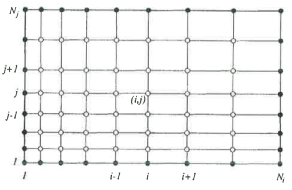
\includegraphics[width=3.0in]{numericalGrid.png}
\captionof{figure}{To solve for the velocity and pressure of water flowing within the pipe, first we need to divide the pipe into a finite set of points. We are interested in the value of velocity and pressure at these points.}
\label{fig:grid}
\end{figure}

\subsubsection{Finite Differences}

Finite difference methods are an approximation to the derivative.
Given some function $u(x)$, if we are interested in the derivative of $u(x)$ at some point $i$ along the x-axis, we could approximate the derivative as follows:

\begin{equation}
\frac{du}{dx} = \frac{u(i + \Delta{x}) - u(i)}{\Delta{x}}
\label{eq:FD}
\end{equation}

This gives the rate of change in $u$ with respect to $x$.
This particular approximation is a \textit{forward approximation} because we are approximating the derivative at $i$ by considering values of $u$ in the forward direction.
The \textit{backwards approximation} is a similar expression, but we are taking the derivative with respect to points to the left of $i$ on the x-axis.

\begin{equation}
\frac{du}{dx} = \frac{u(i) - u(i - \Delta{x})}{\Delta{x}}
\label{eq:BD}
\end{equation}

A central difference about the point $i$ would be observing the change in $u$ from $i - \Delta{x}$ to $i + \Delta{x}$:

\begin{equation}
\frac{du}{dx} = \frac{u(i + \Delta{x}) - u(i - \Delta{x})}{2\Delta{x}}
\label{eq:CD}
\end{equation}

\begin{figure}
\centering
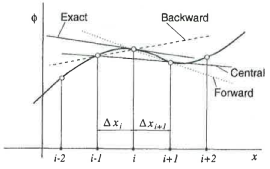
\includegraphics[width=3.0in]{finiteDif.png}
\captionof{figure}{The forward, backward and central differences are approximations to the actual derivative of our function. Some approximations will be better than others, depending on the function in consideration.}
\label{fig:difs}
\end{figure}

The factor of $2\Delta{x}$ in the central difference comes about beause we are observing the change in $u$ over twice the distance utilized in the forward and backward difference equations.

\subsubsection{Finite Difference from Taylor Series}
If we want to be a little more specific in our expression for the forward, backward, central differences, we can express them using the Taylor Series.
The Taylor Series expansion of our function $u(x)$ centered at the point $i$ is the following:

\begin{equation}
u(x) = u(x_i) + (x-x_i)\bigg(\frac{\partial{u}}{\partial{x}}\bigg)_i + \frac{(x-x_i)^2}{2}\bigg(\frac{\partial^2{u}}{\partial{x^2}}\bigg)_i + \frac{(x-x_i)^3}{6}\bigg(\frac{\partial^3{u}}{\partial{x^3}}\bigg)_i + ... + \frac{(x-x_i)^n}{n!}\bigg(\frac{\partial^n{u}}{\partial{x^n}}\bigg)_i + H 
\end{equation}

The $H$ in our expression stands for the \textit{higher order terms}, the product of the higher order derivatives and the displacement between $x$ and $i$.
Thus we can solve for the first derivative of $u$ with respect to $x$, $(\frac{\partial{u}}{\partial{x}})_i$:

\begin{equation}
\bigg(\frac{\partial{u}}{\partial{x}}\bigg)_i = \frac{u(x) - u(i)}{x-i}
- \frac{(x-i)^2}{2}\bigg(\frac{\partial^2{u}}{\partial{x^2}}\bigg)_i - \frac{(x-i)^3}{6}\bigg(\frac{\partial^3{u}}{\partial{x^3}}\bigg)_i - ... - \frac{(x-i)^n}{n!}\bigg(\frac{\partial^n{u}}{\partial{x^n}}\bigg)_i + H 
\end{equation}

If $x$ is sufficiently close to $i$, the higher order terms will tend to zero and we can be satisfied with the following expression, which is a \textit{first order approximation} to the derivative of $u$ with respect to $x$ at the point $i$:

\begin{equation}
\bigg(\frac{\partial{u}}{\partial{x}}\bigg)_i \approx \frac{u(x) - u(x_i)}{x-x_i}
\end{equation}

Returning to our numerical grid, if we keep our expansion centered at the point $x_i$ and let $x = x_{i+1}$, our Taylor Series Expansion becomes:

\begin{equation}
u(x_{i+1}) = u(x_{i}) + (x_{i+1}-x_{i})\bigg(\frac{\partial{u}}{\partial{x}}\bigg)_i + \frac{(x_{i+1}-x_{i})^2}{2}\bigg(\frac{\partial^2{u}}{\partial{x^2}}\bigg)_i + \frac{(x_{i+1}-x_{i})^3}{6}\bigg(\frac{\partial^3{u}}{\partial{x^3}}\bigg)_i + ... + \frac{(x_{i+1}-x_{i})^n}{n!}\bigg(\frac{\partial^n{u}}{\partial{x^n}}\bigg)_i + H 
\end{equation}

Solving for $(\frac{\partial{u}}{\partial{x}})_i$  we have an expression equivalent to the forward difference derivative we found above (\ref{eq:FD}):

\begin{equation}
\bigg(\frac{\partial{u}}{\partial{x}}\bigg)_i \approx \frac{u(x_{i+1}) - u(x_i)}{\Delta{x}}
\end{equation}

So, we have found our forward difference equation concretely, that is, we have the first order approximation and knowledge of the higher order terms as well.
The higher order terms that we dropped will eventually be a source of error that we will have to keep track of later. 
By applying the above process to the pairs of points $x_i$ and $x_{i-1}$, as well as $x_{i+1}$ and $x_{i-1}$ we can obtain the backward difference formula and central difference formula, respectively, from the Taylor Series Expansion.

\begin{equation}
\bigg(\frac{\partial{u}}{\partial{x}}\bigg)_i \approx \frac{u(x_{i}) - u(x_{i-1})}{\Delta{x}}
\end{equation}

\begin{equation}
\bigg(\frac{\partial{u}}{\partial{x}}\bigg)_i \approx \frac{u(x_{i+1}) - u(x_{i-1})}{\Delta{x}}
\end{equation}

\subsubsection{Finite Difference: Second Derivative}

Coming soon...


\end{document}

